\section{\faWrench\ Retrieval Augmented Generation\\{\small Parte 1}} % (fold)
\label{sec:spring-ai-rag-part-1}
%
\begin{frame}[t,fragile] \frametitle{Progetto Spring AI}
    \framesubtitle{Applicazione e passaggi}
    {\small
    \begin{itemize}[leftmargin=10pt,align=right]
        \onslide<1->\item[\alert{\faArrowCircleRight}] \textit{Chatbot} Ollama-CV e Gemini-Venis
        \onslide<2->\item[\faExclamationTriangle] Approccio \textit{naive} (informazione testuale estratta tramite GENAI-\textit{assisted} \textit{web scraping}/\textit{summarization})
        \begin{itemize}[leftmargin=10pt,align=right]
            \onslide<2->\item[\alertedcircled{1}] Iscrizione al portale HuggingFace e creazione \textit{access token}
            \onslide<3->\item[\alertedcircled{2}] Verifica e modifica variabili di ambiente
            \onslide<4->\item[\alertedcircled{3}] Creazione configurazione ambiente Docker Qdrant
            \onslide<5->\item[\alertedcircled{4}] Modifica dipendenze di progetto
            \onslide<6->\item[\alertedcircled{5}] Modifica configurazione applicativo
            \onslide<7->\item[\alertedcircled{6}] Creazione \textit{prompt templates} per strategia RAG
            \onslide<8->\item[\alertedcircled{7}] Configurazione \textit{vector store} per Ollama e Gemini \textit{embeddings}
            \onslide<9->\item[\alertedcircled{8}] Creazione \textit{component} per popolamento \textit{vector store} (dati Venis e CV)
            \onslide<10->\item[\alertedcircled{9}] Creazione interfaccia e implementazione del servizio
            \onslide<11->\item[\alertedcircled{10}] Modifica controllore MVC
            \onslide<12->\item[\alertedcircled{11}] \textit{Test} delle funzionalità con Postman/Insomnia
        \end{itemize}
    \end{itemize}
    }
\end{frame}
%
\begin{frame}[t,fragile] \frametitle{Ambiente di sviluppo}
\framesubtitle{Creazione account HuggingFace}
	\vspace*{-.5cm}
    {\footnotesize
    \begin{itemize}
        \only<1|handout:1>{\item[\alertedcircled{1}] Accedere al portale \url{https://huggingface.co/} e cliccare il pulsante \texttt{Sign up}}
        \only<2|handout:2>{\item[\alertedcircled{2}] Creare una nuova utenza}
        \only<3|handout:3>{\item[\alertedcircled{3}] Accedere al portale e selezionare \texttt{Access Tokens} nel menu in alto a destra}
        \only<4|handout:4>{\item[\alertedcircled{4}] Premere sul pulsante \texttt{Create new token}}
        \only<5|handout:5>{\item[\alertedcircled{5}] Selezionare \textit{token} di tipo \texttt{Write}, denominare il \textit{token} e premere \texttt{Create token}}
        \only<6-7|handout:6-7>{\item[\alertedcircled{6}] Cercare il modello di \textit{embedding}, leggendone la \textit{card}} 
    \end{itemize}
    }
    \vfill
    \begin{minipage}[b]{\textwidth}
		\centering
        \only<1|handout:1>{
		    \begin{figure}[ht]
			    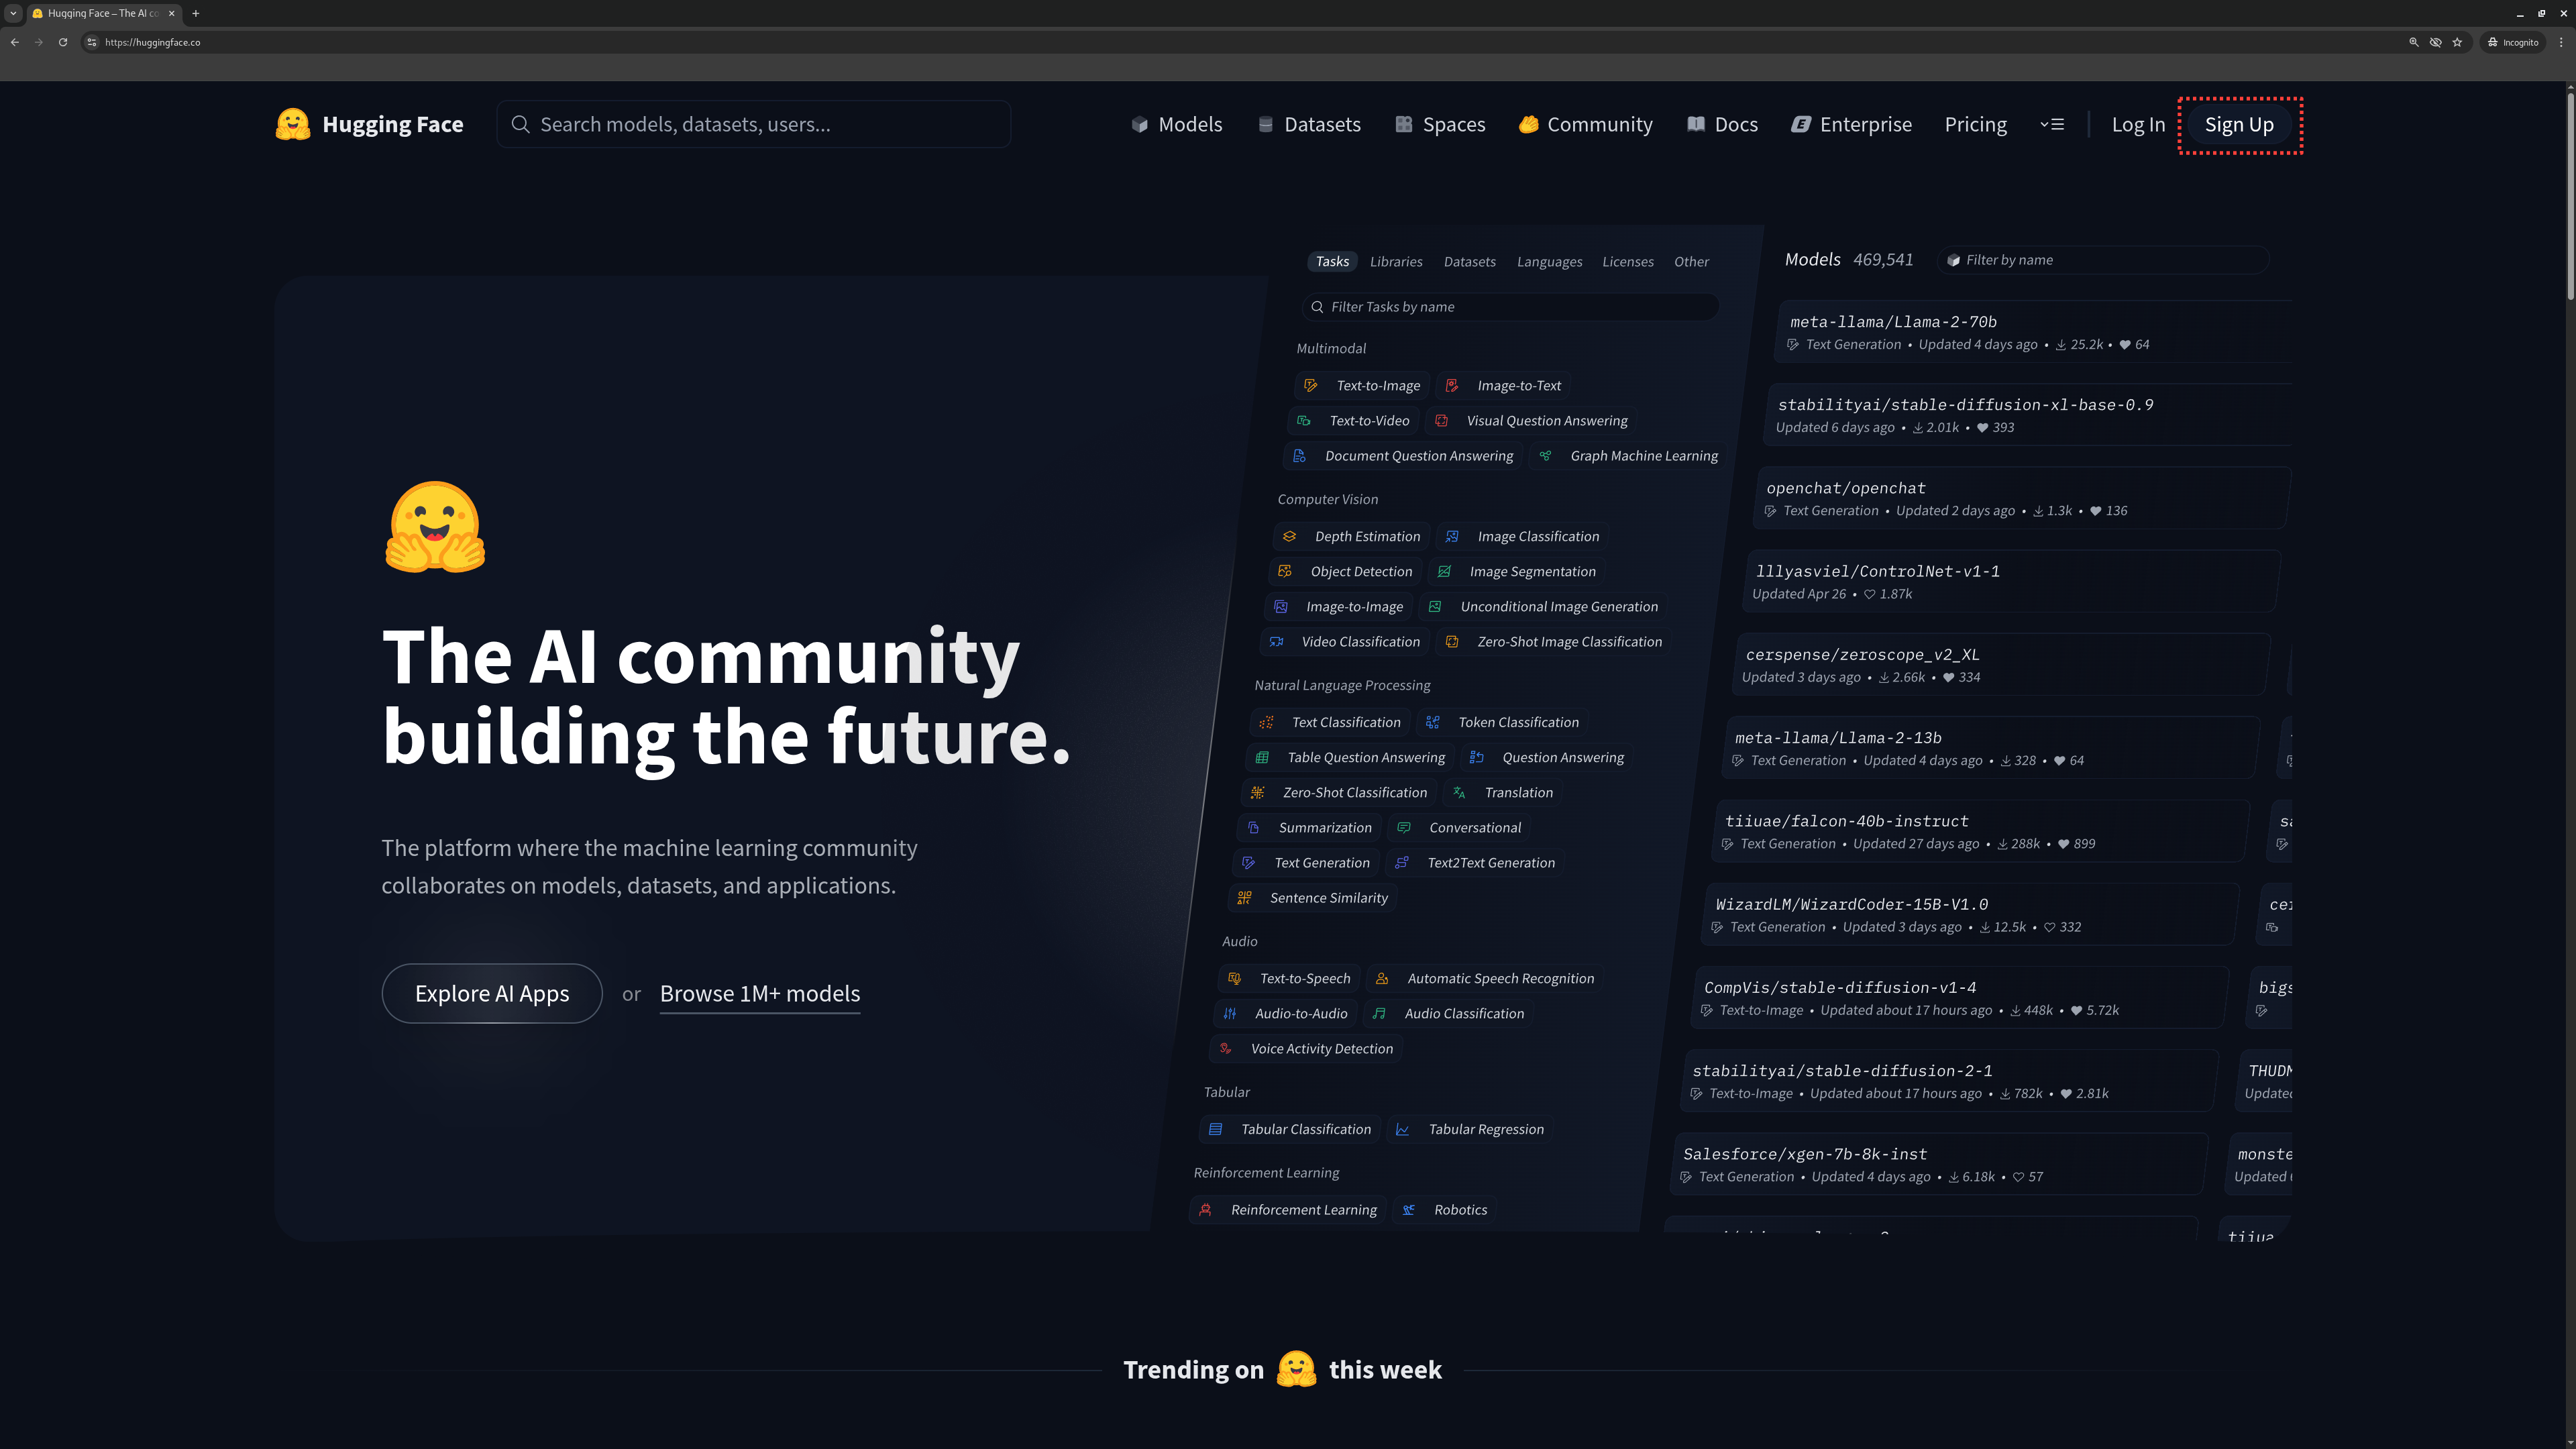
\includegraphics[width=\textwidth, frame]{img/huggingface-portal.png}
		    \end{figure}
        }
        \only<2|handout:2>{
		    \begin{figure}[ht]
			    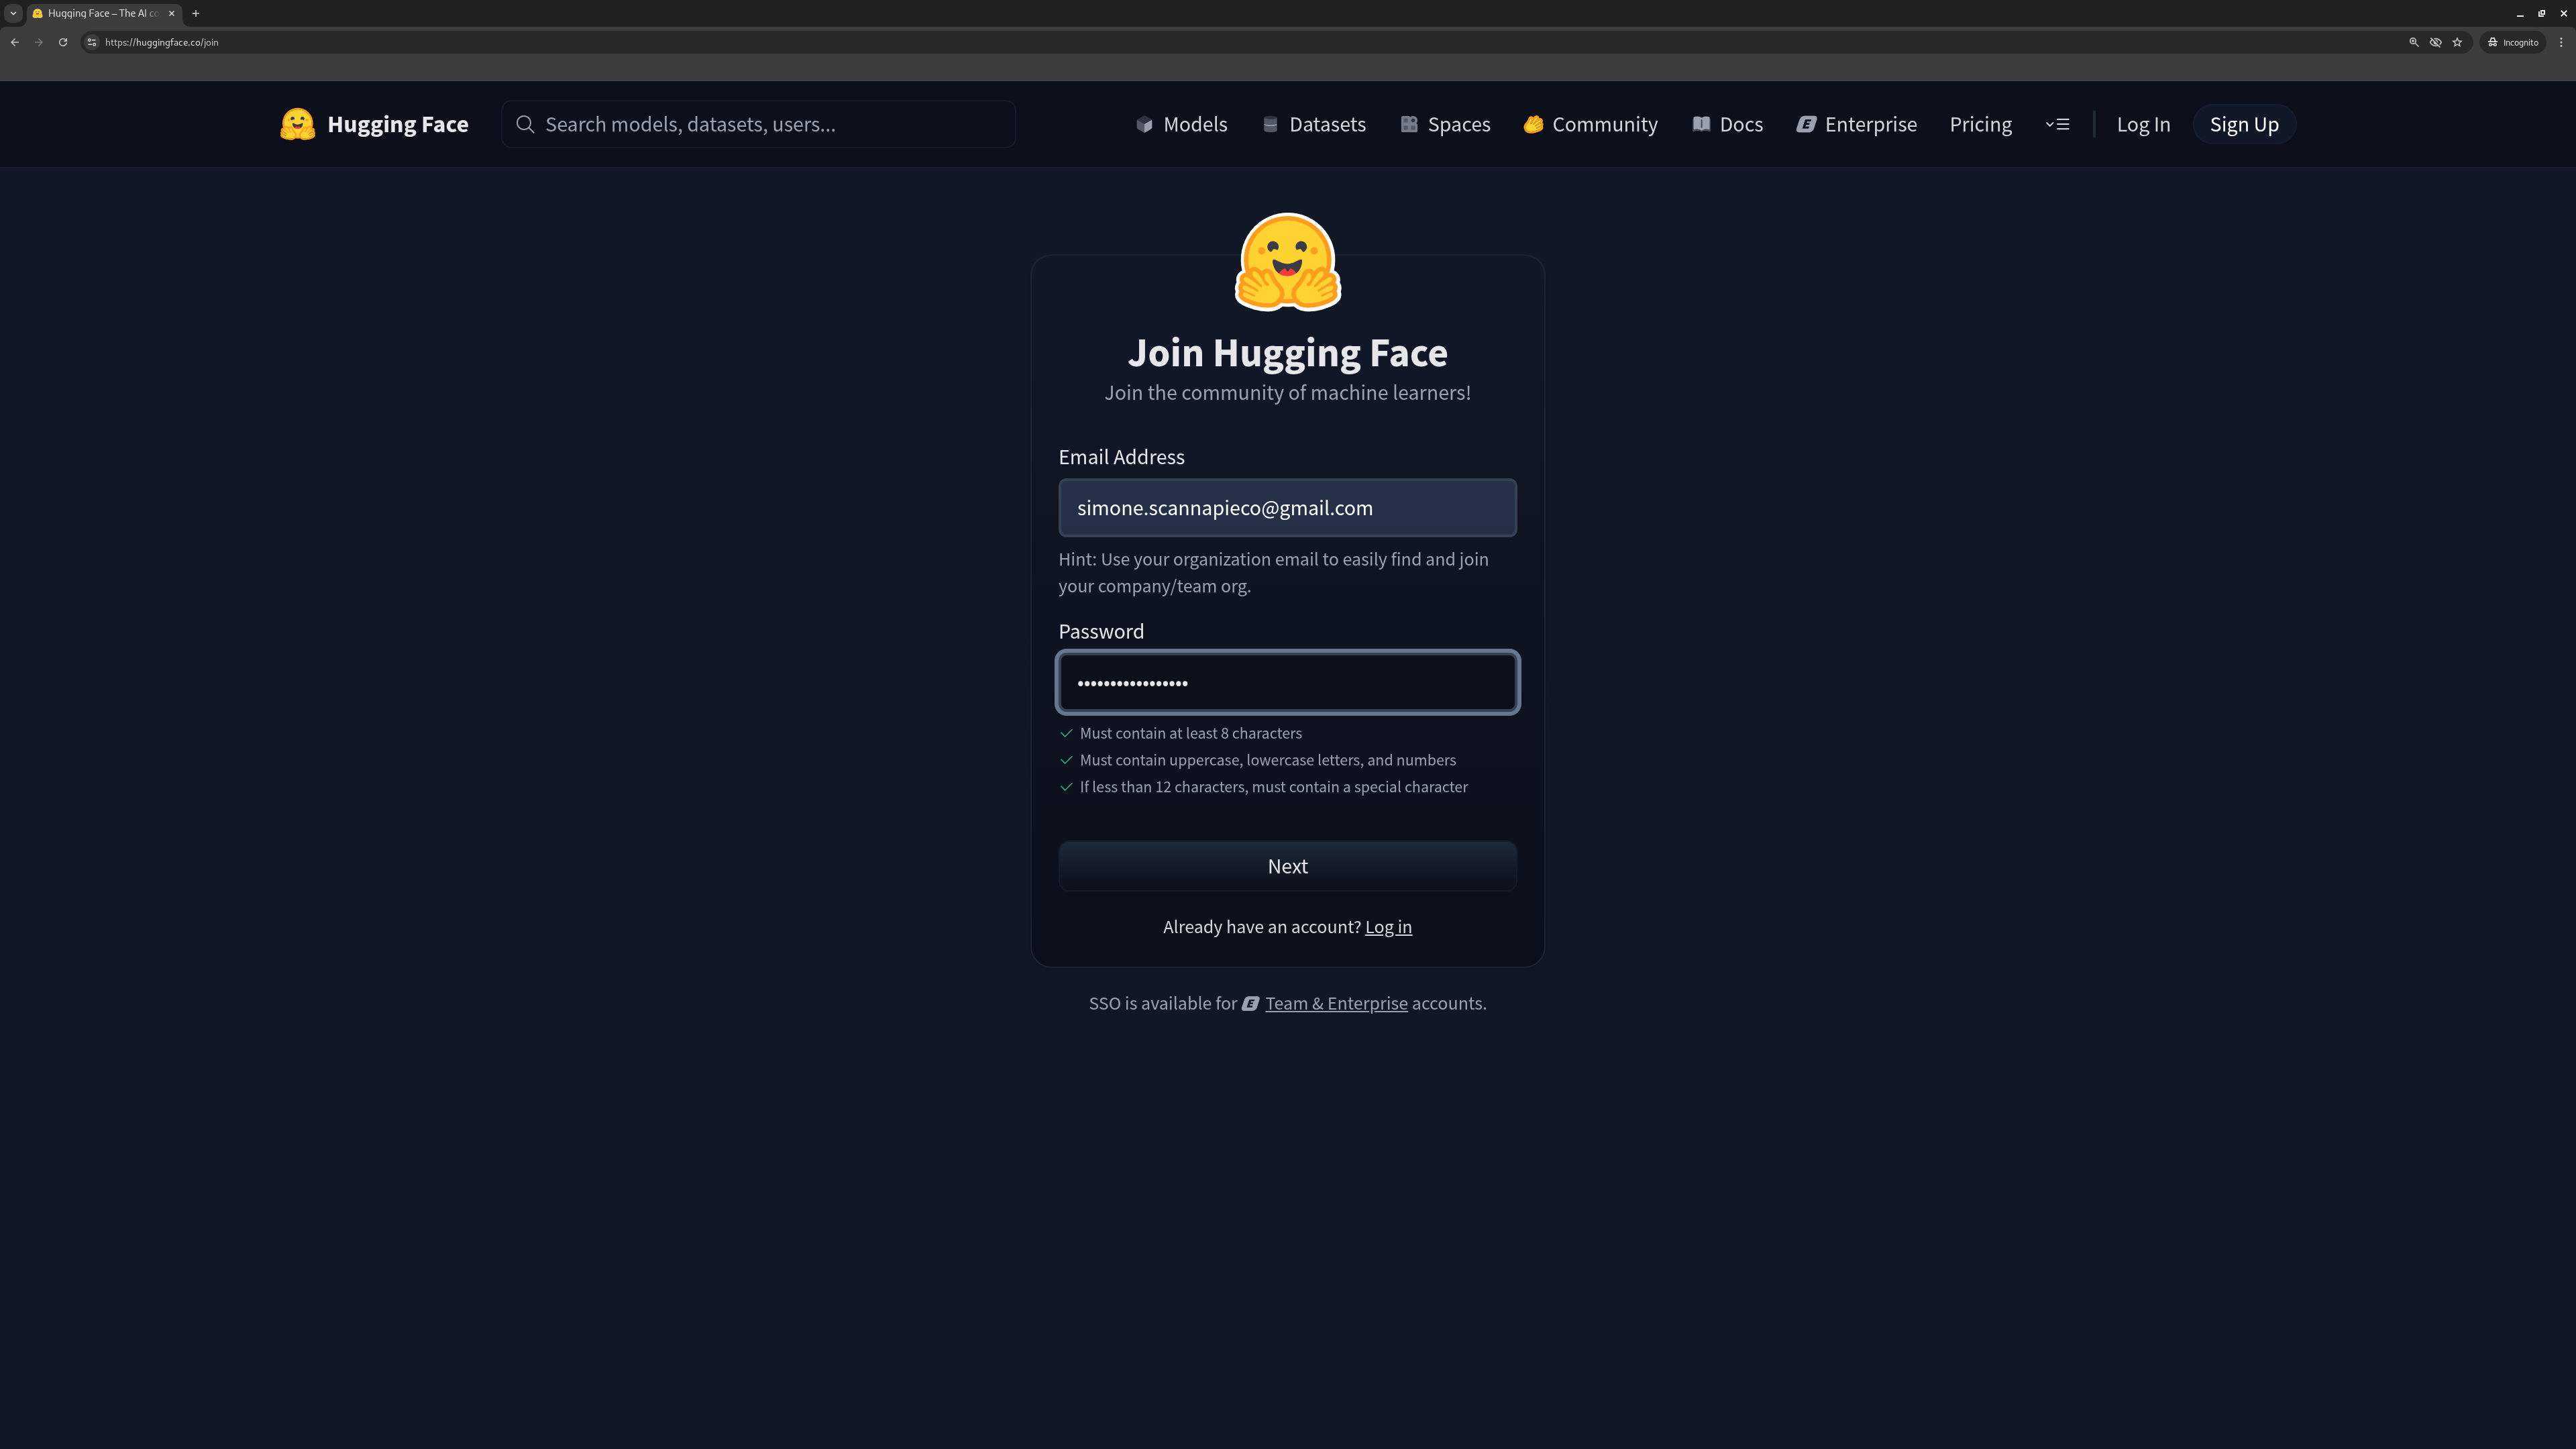
\includegraphics[width=\textwidth, frame]{img/huggingface-portal-sign-up.png}
		    \end{figure}
        }
        \only<3|handout:3>{
		    \begin{figure}[ht]
			    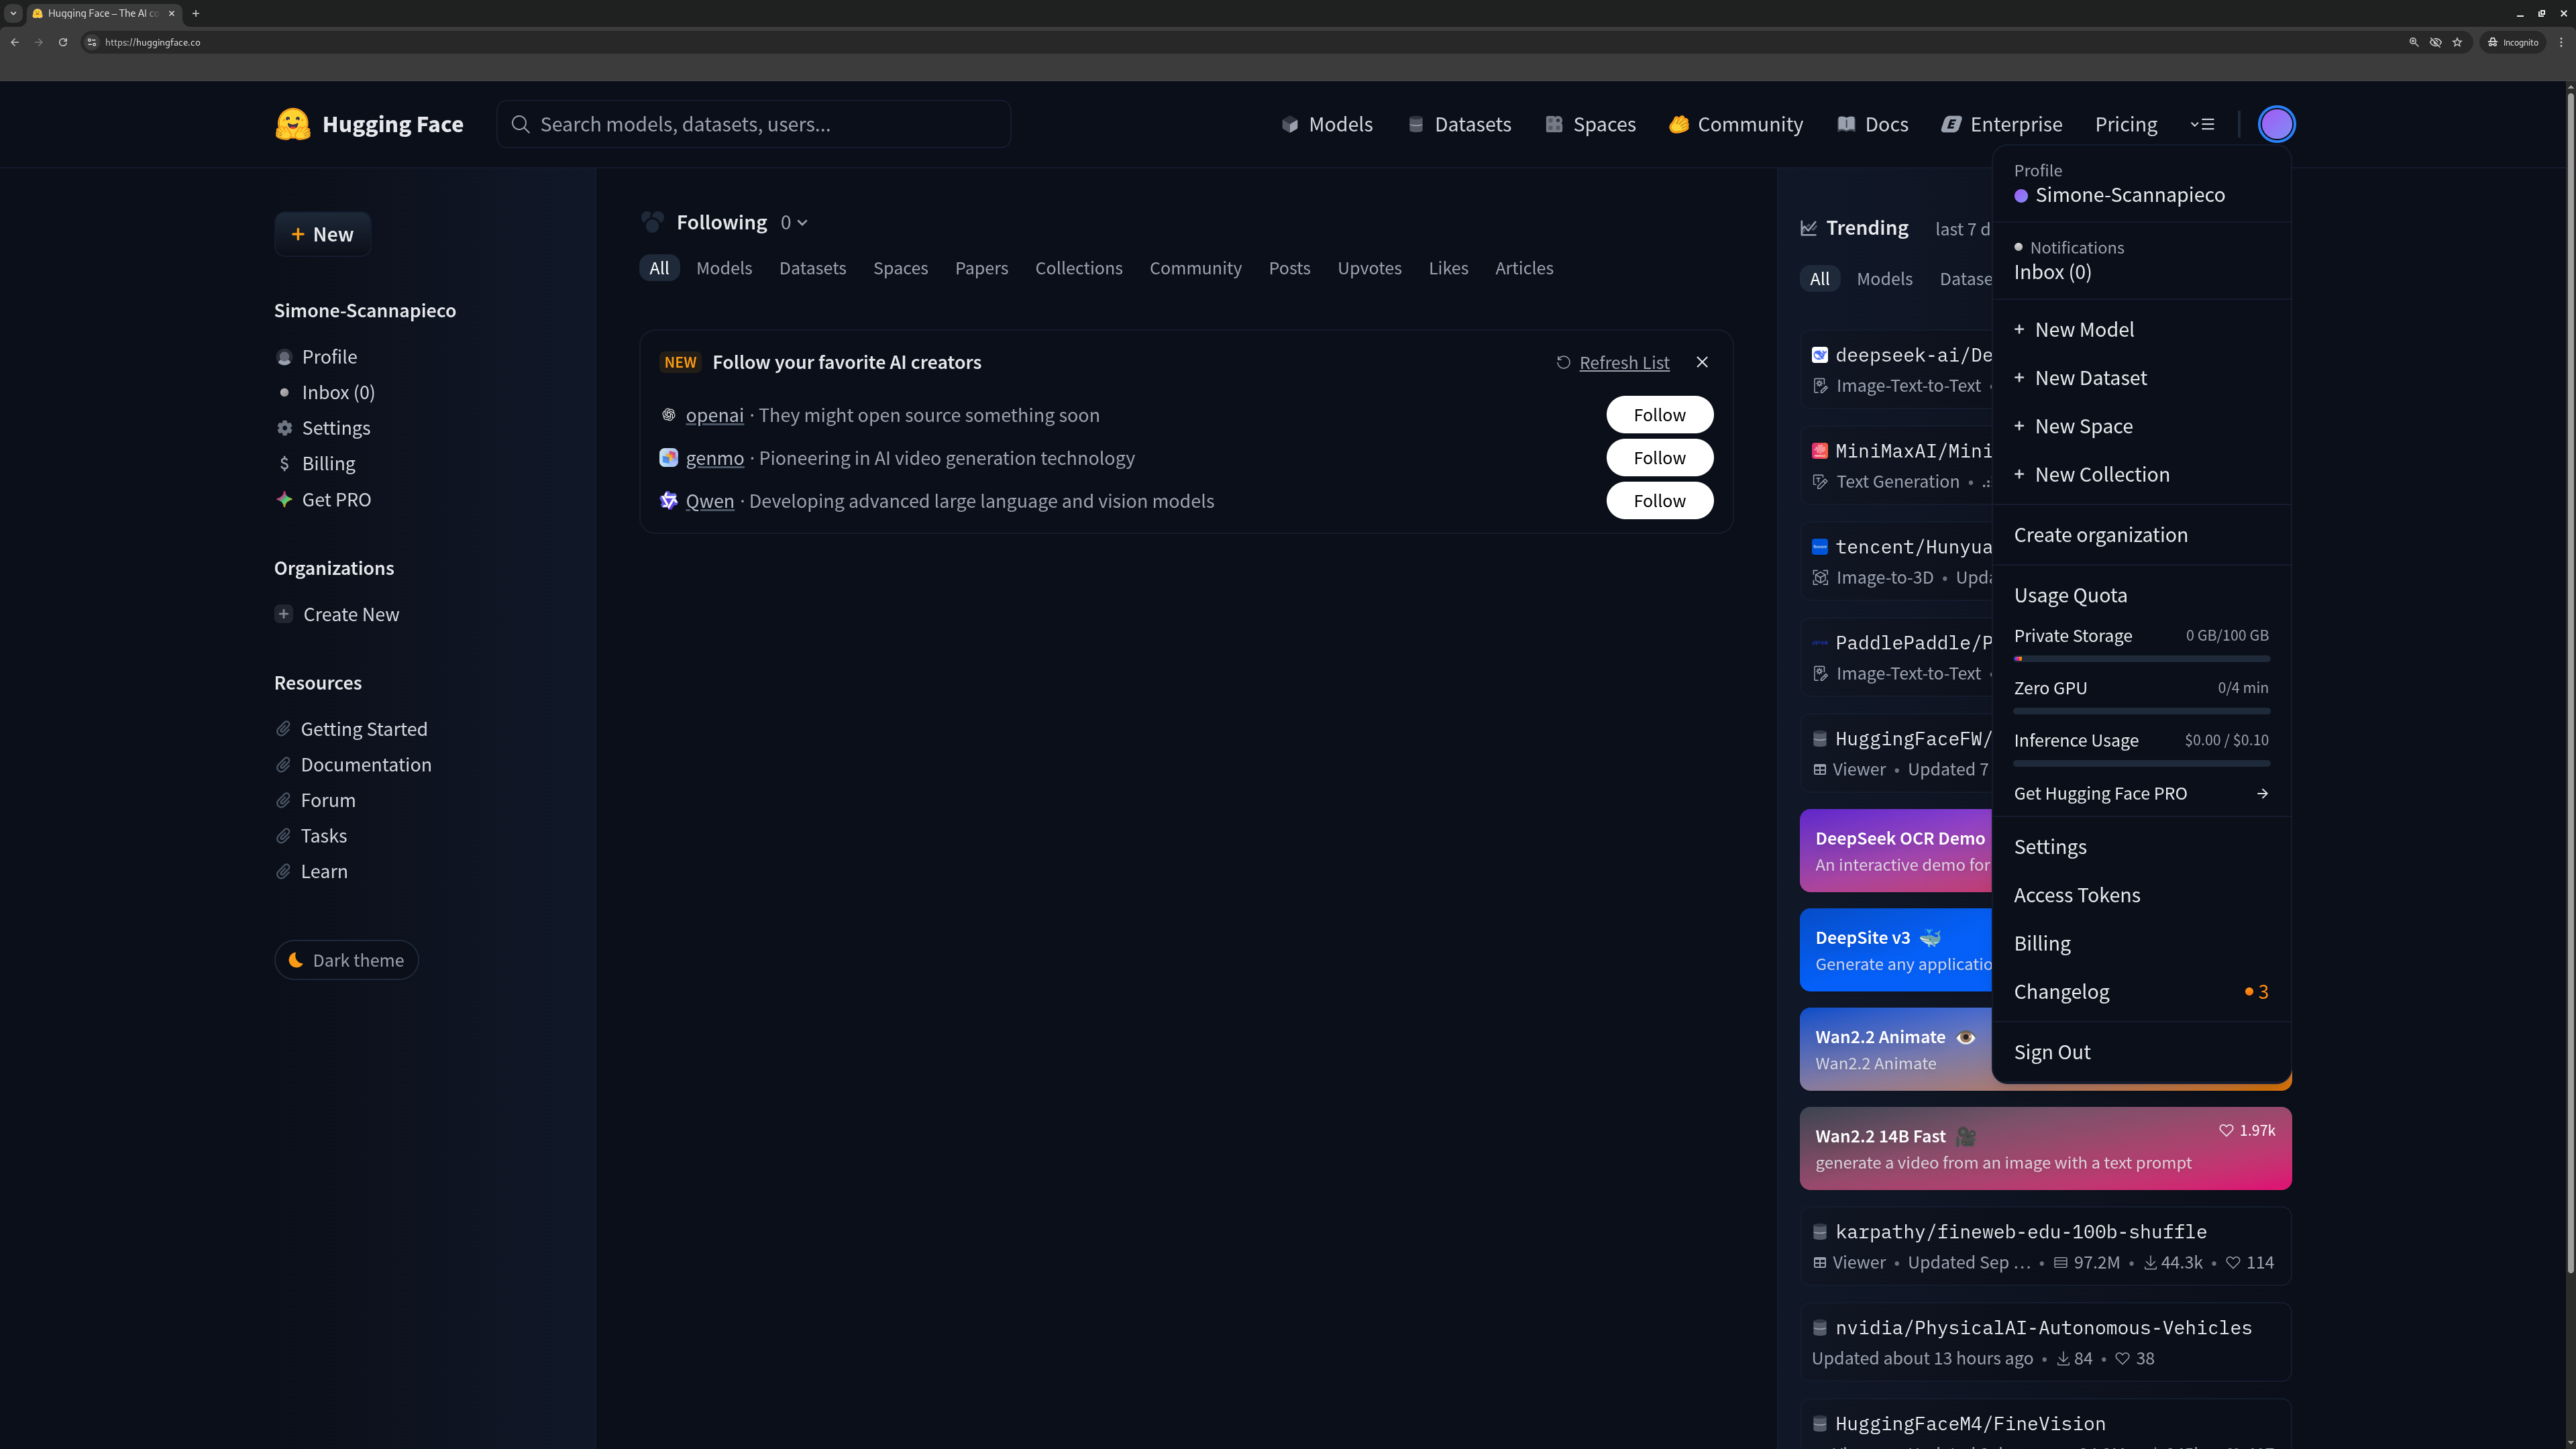
\includegraphics[width=\textwidth, frame]{img/huggingface-portal-access-token.png}
		    \end{figure}
        }
        \only<4|handout:4>{
		    \begin{figure}[ht]
			    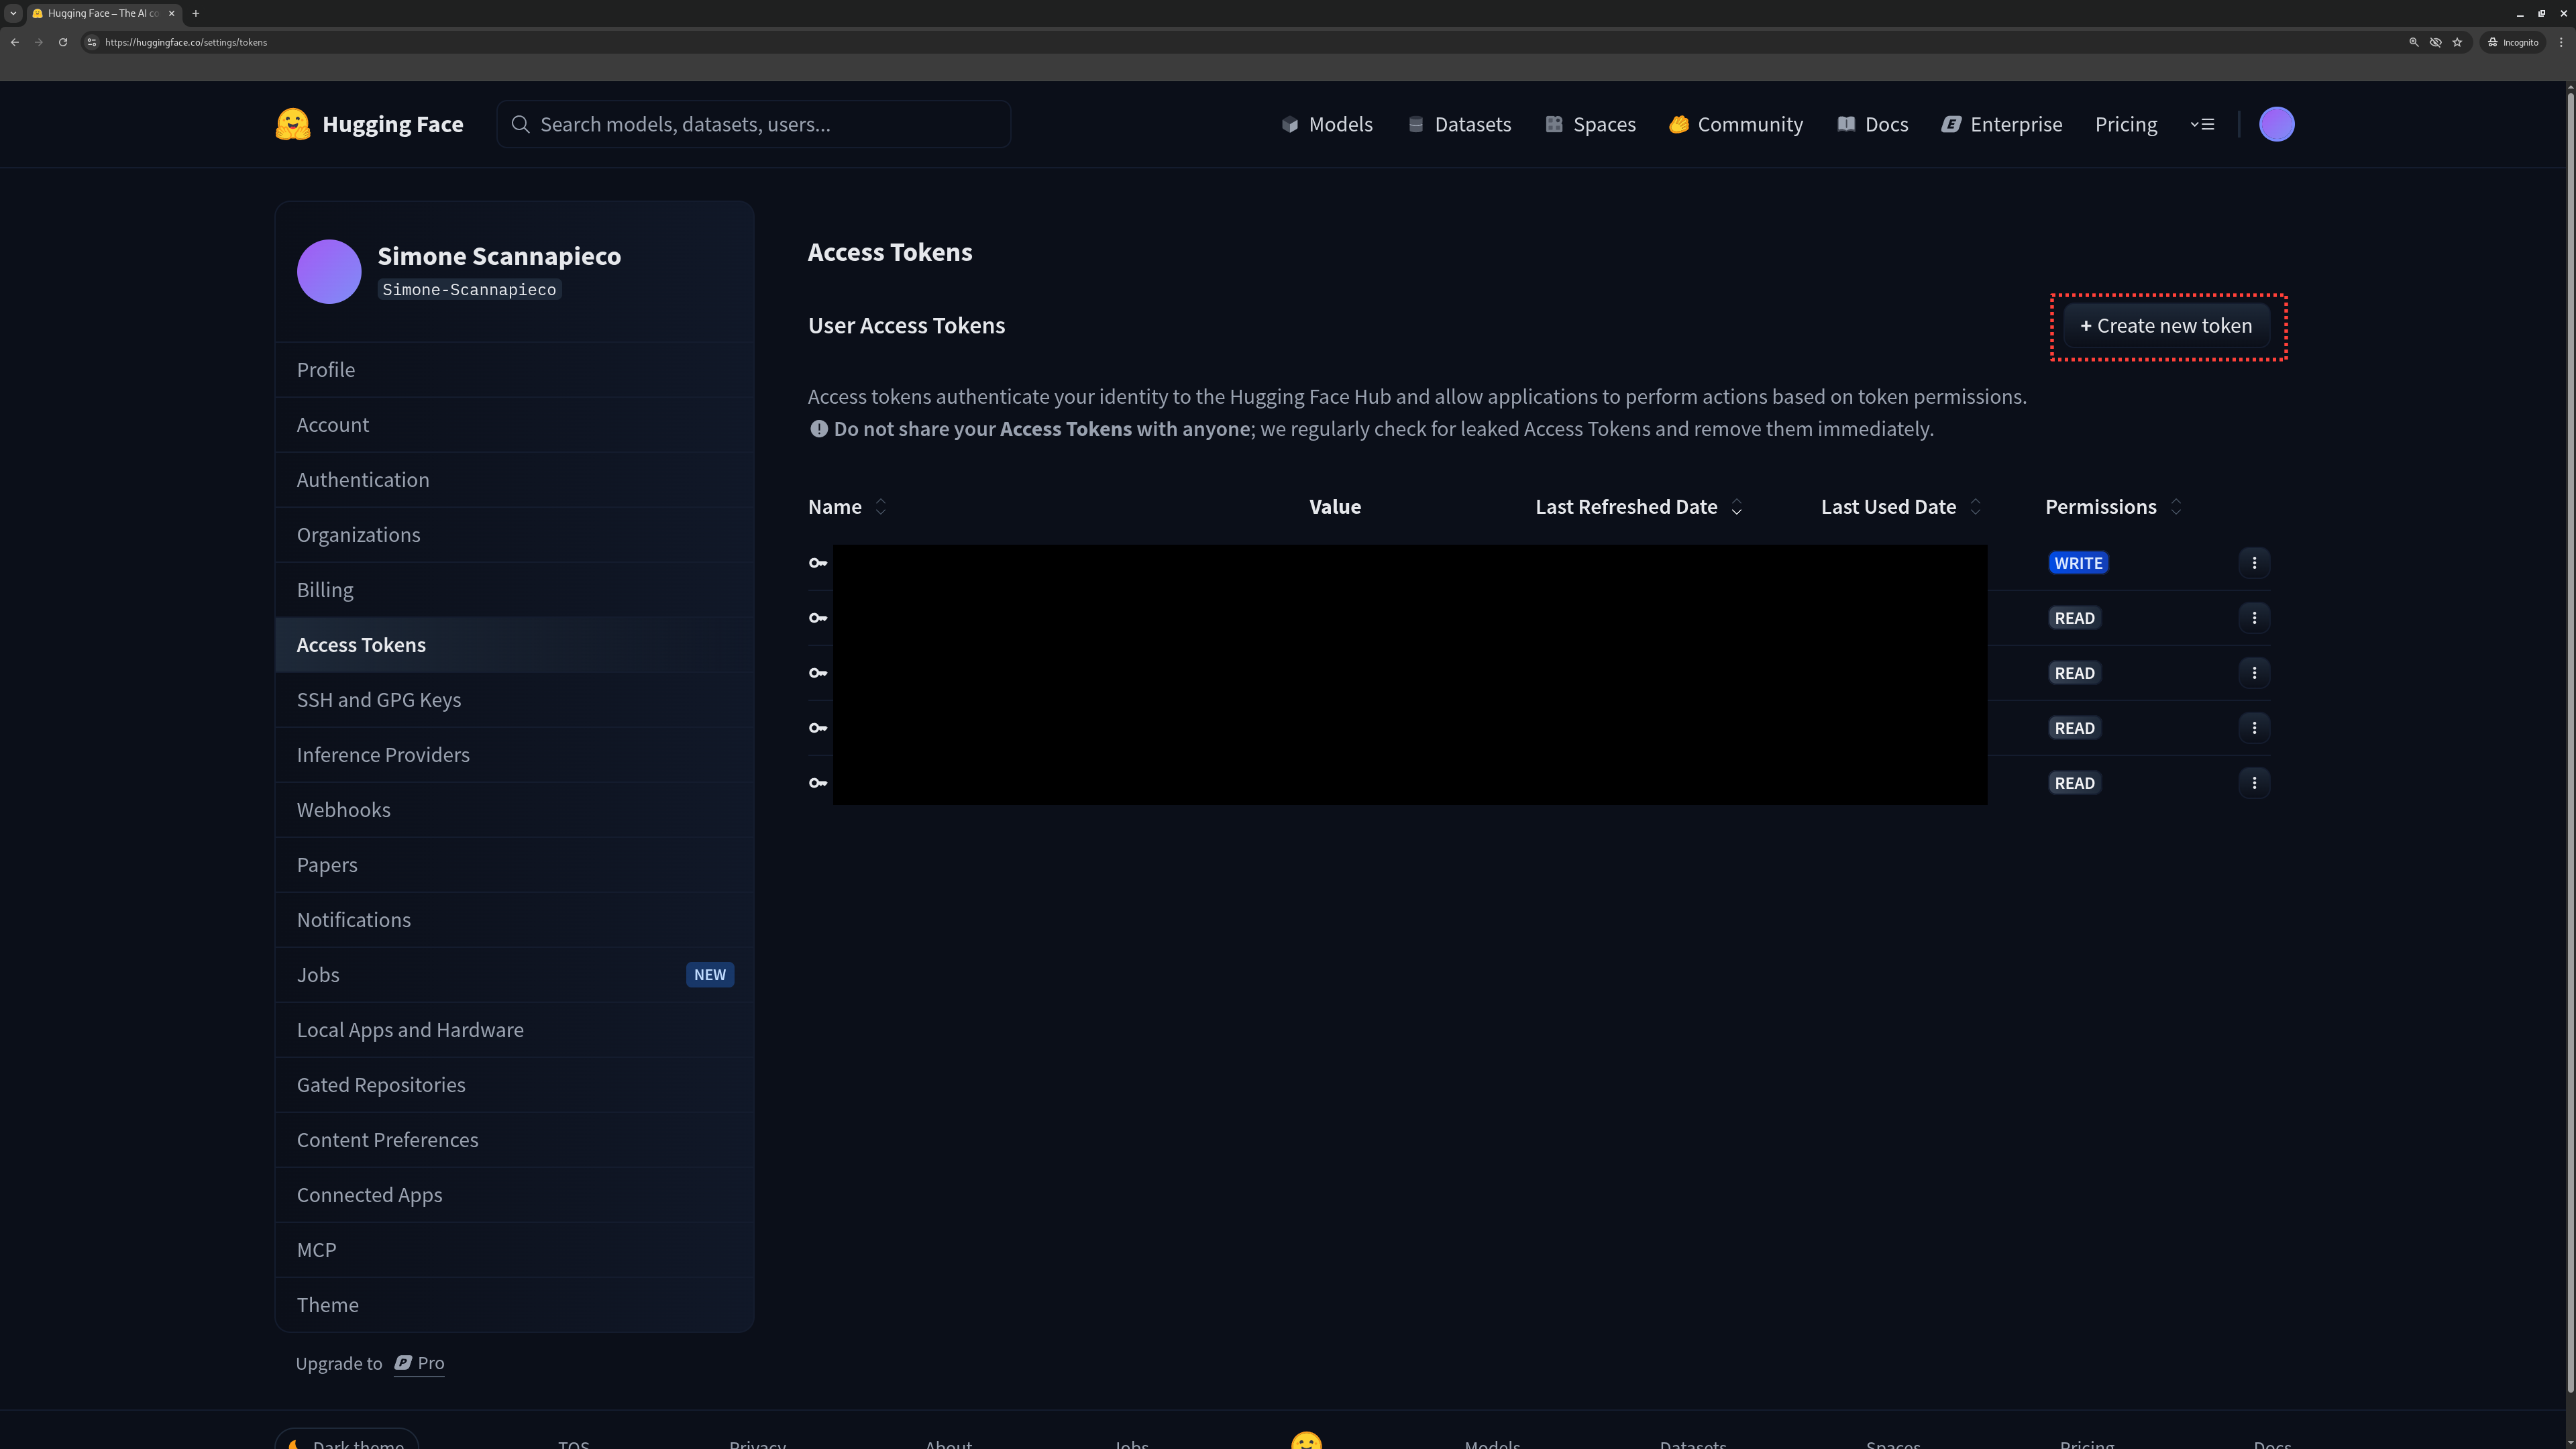
\includegraphics[width=\textwidth, frame]{img/huggingface-portal-access-token-create-new-token.png}
		    \end{figure}
        }
        \only<5|handout:5>{
		    \begin{figure}[ht]
			    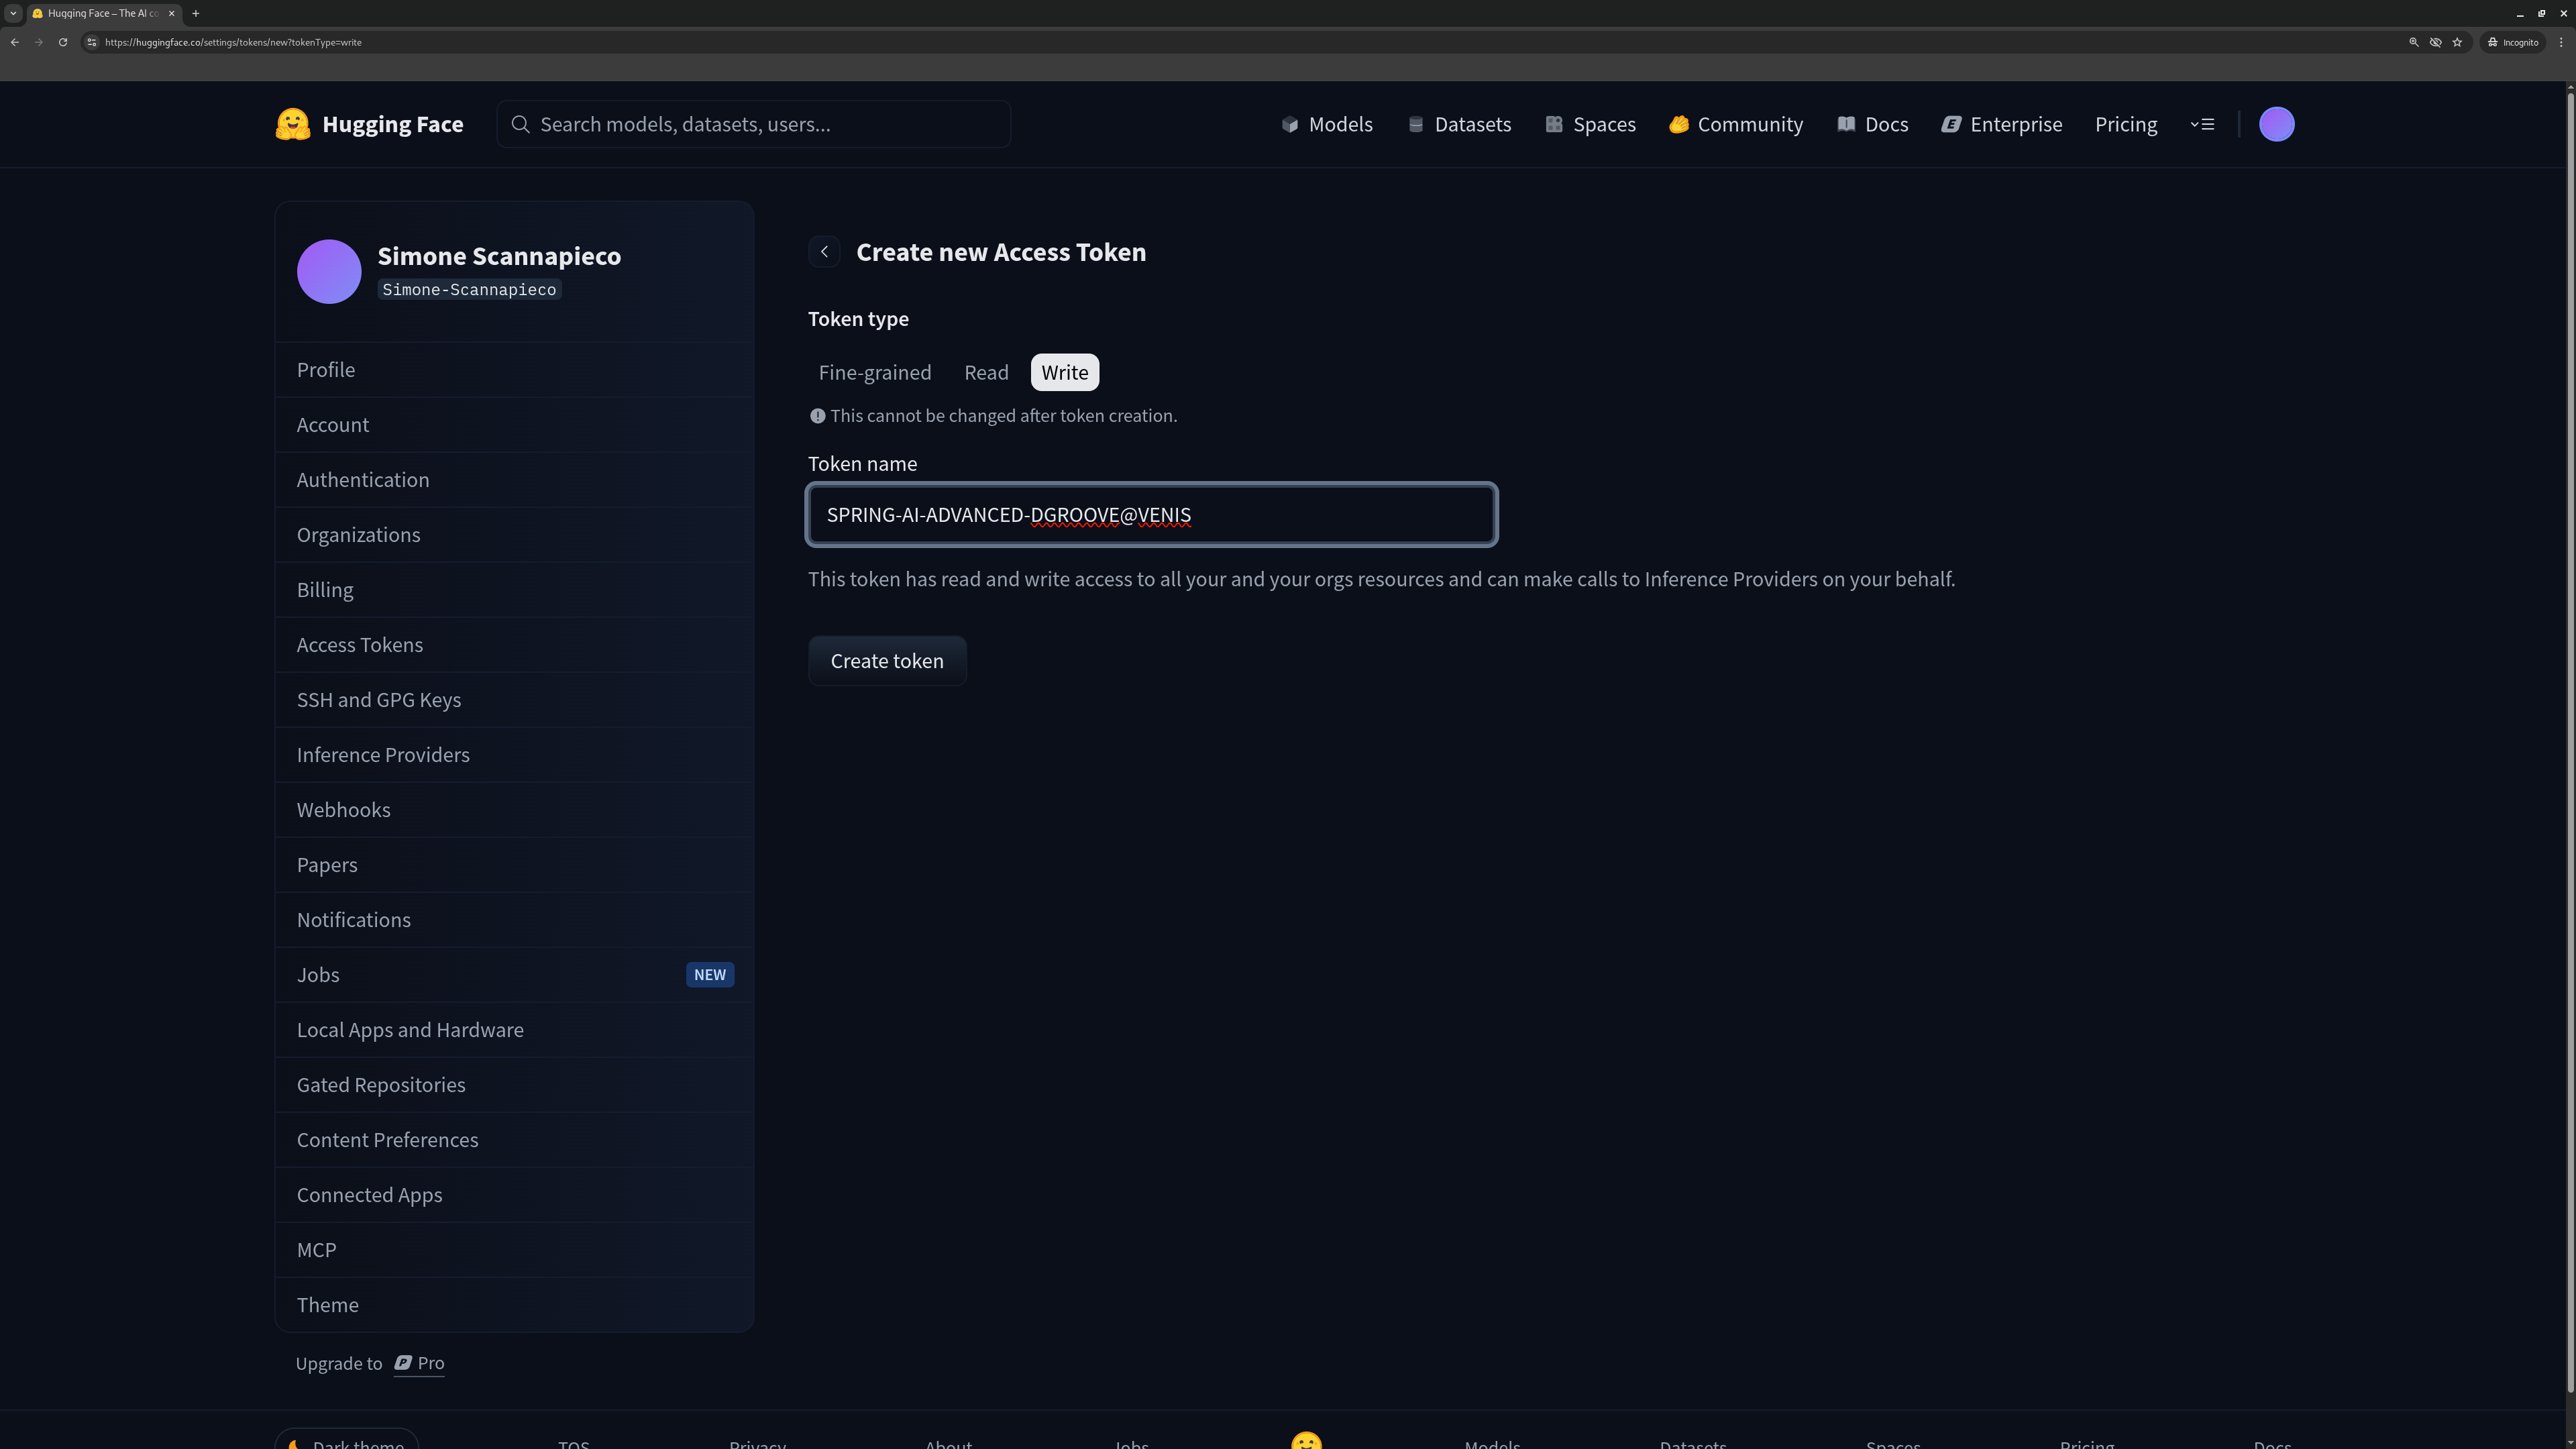
\includegraphics[width=\textwidth, frame]{img/huggingface-portal-access-token-create-write-token.png}
		    \end{figure}
        }
        \only<6|handout:6>{
		    \begin{figure}[ht]
			    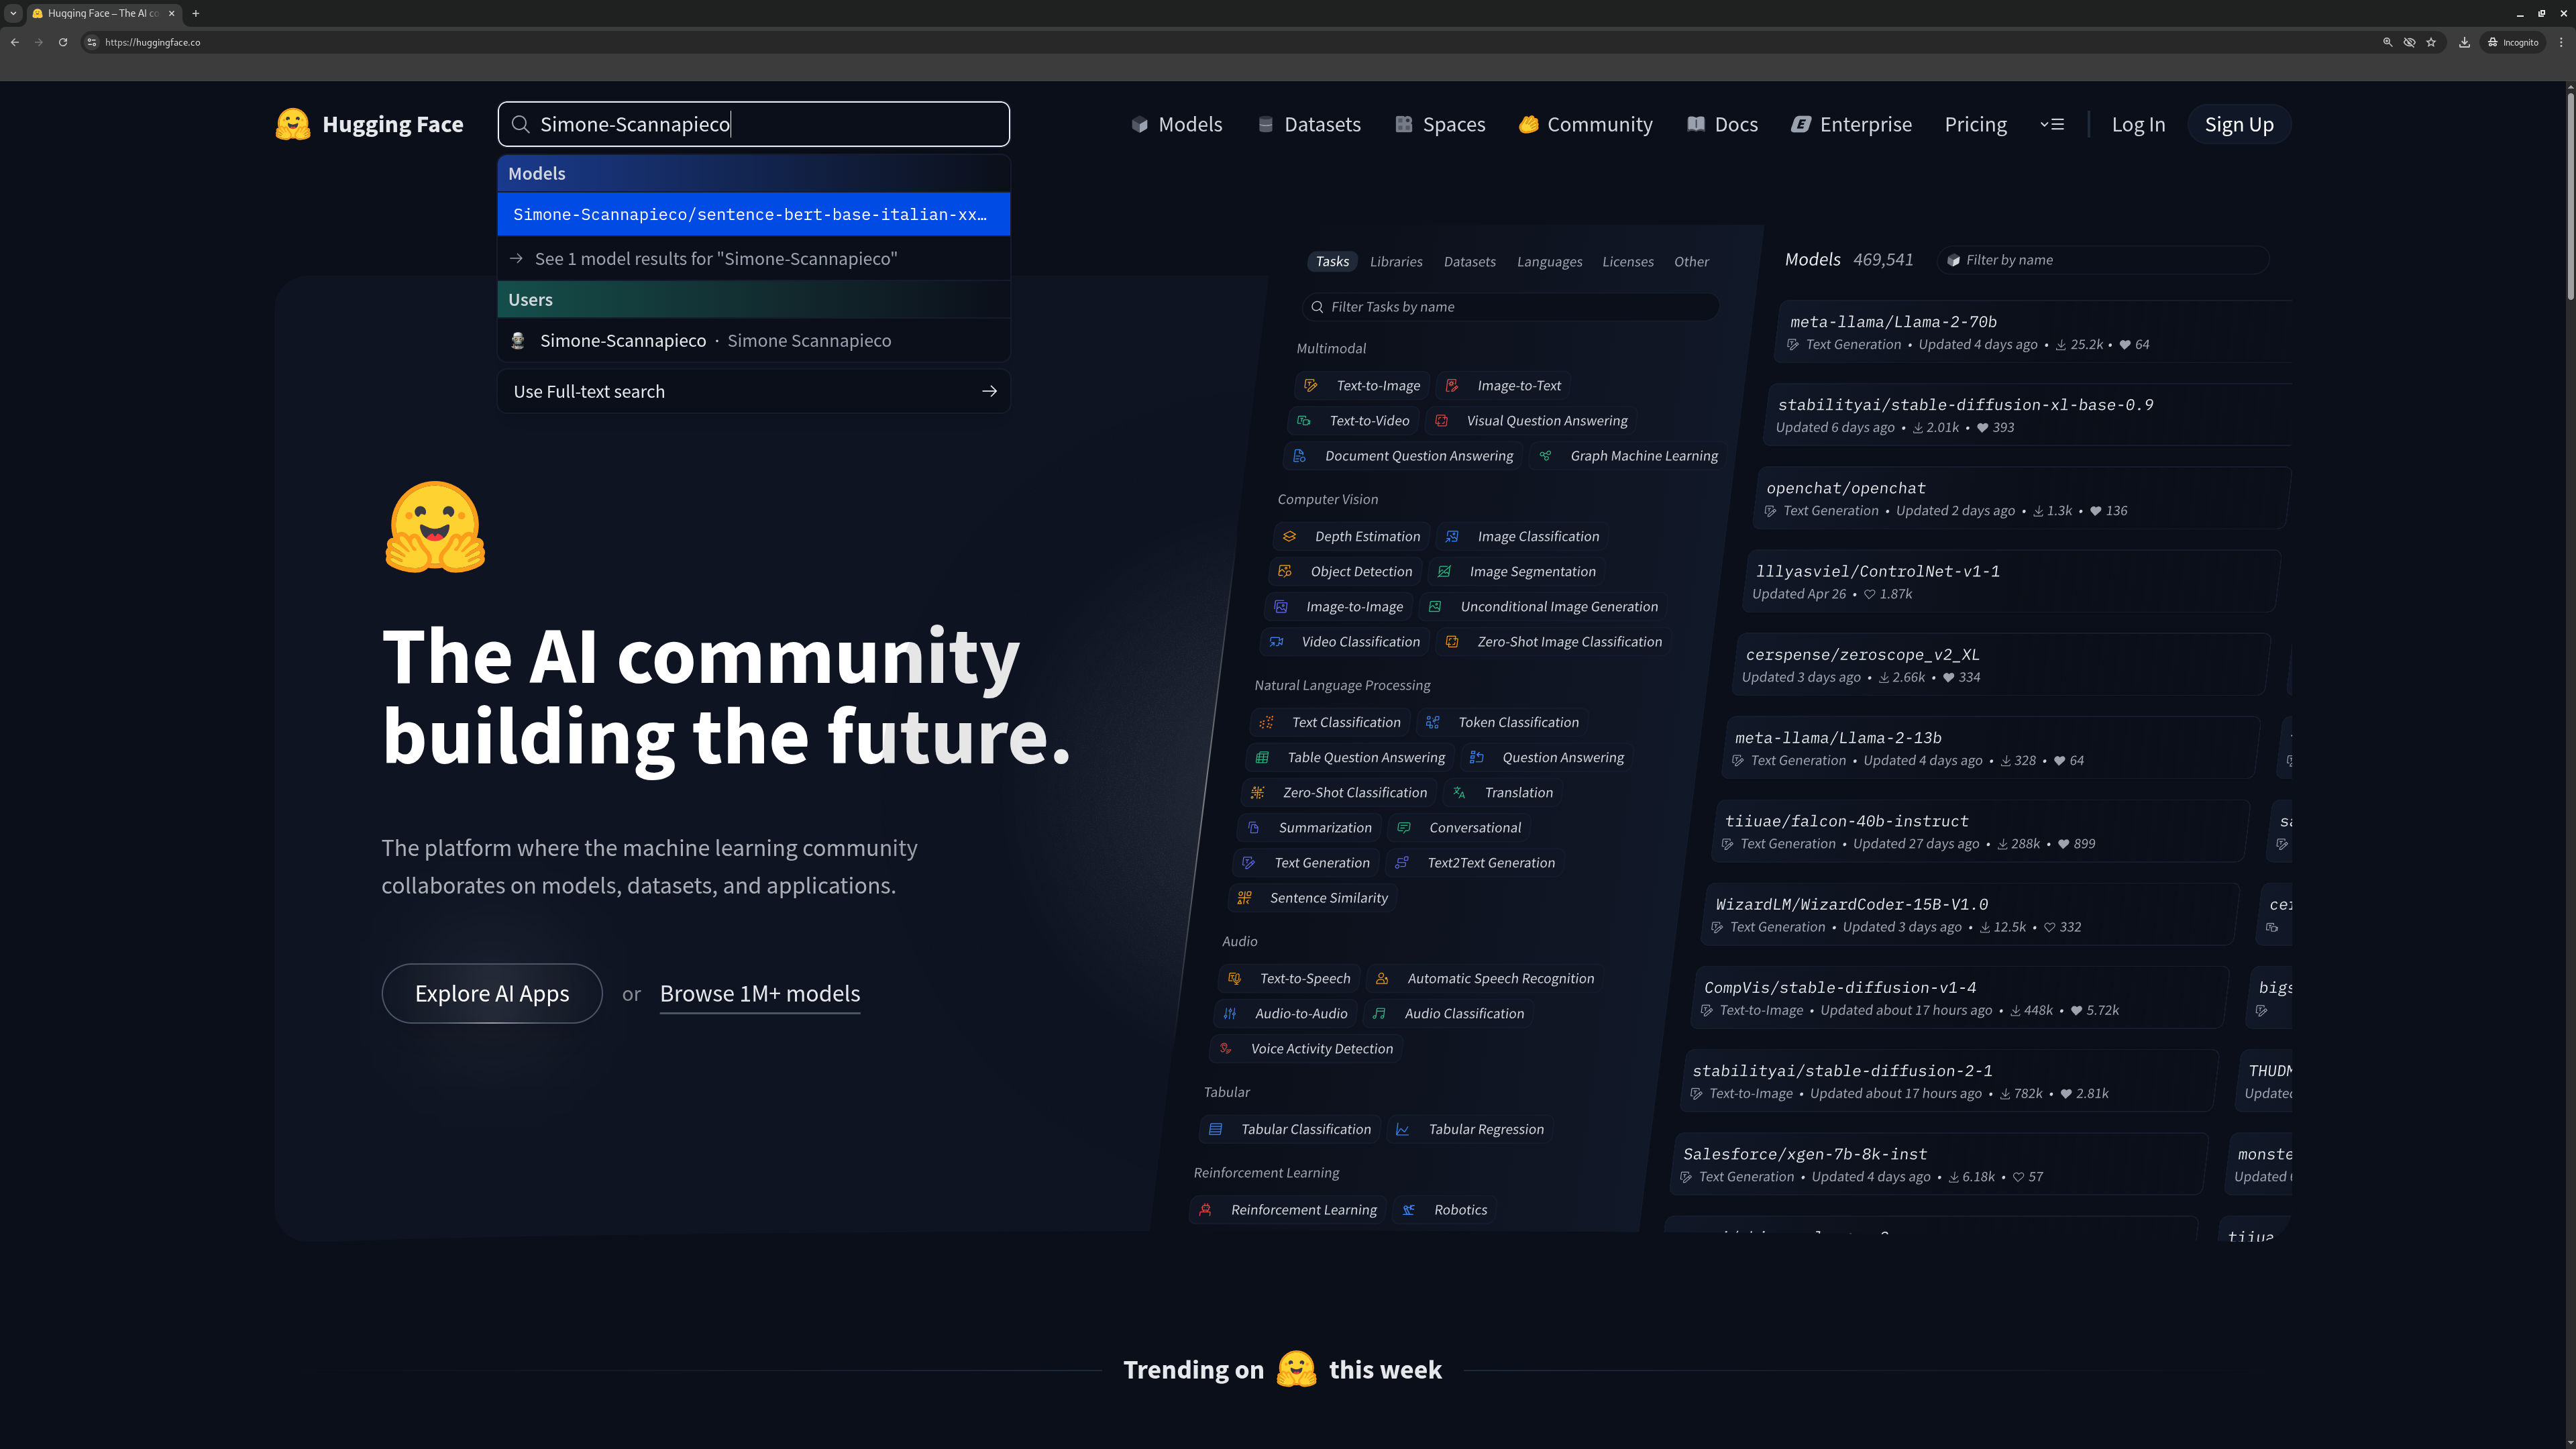
\includegraphics[width=\textwidth, frame]{img/huggingface-search-bert-ita.png}
		    \end{figure}
        }
        \only<7|handout:7>{
		    \begin{figure}[ht]
			    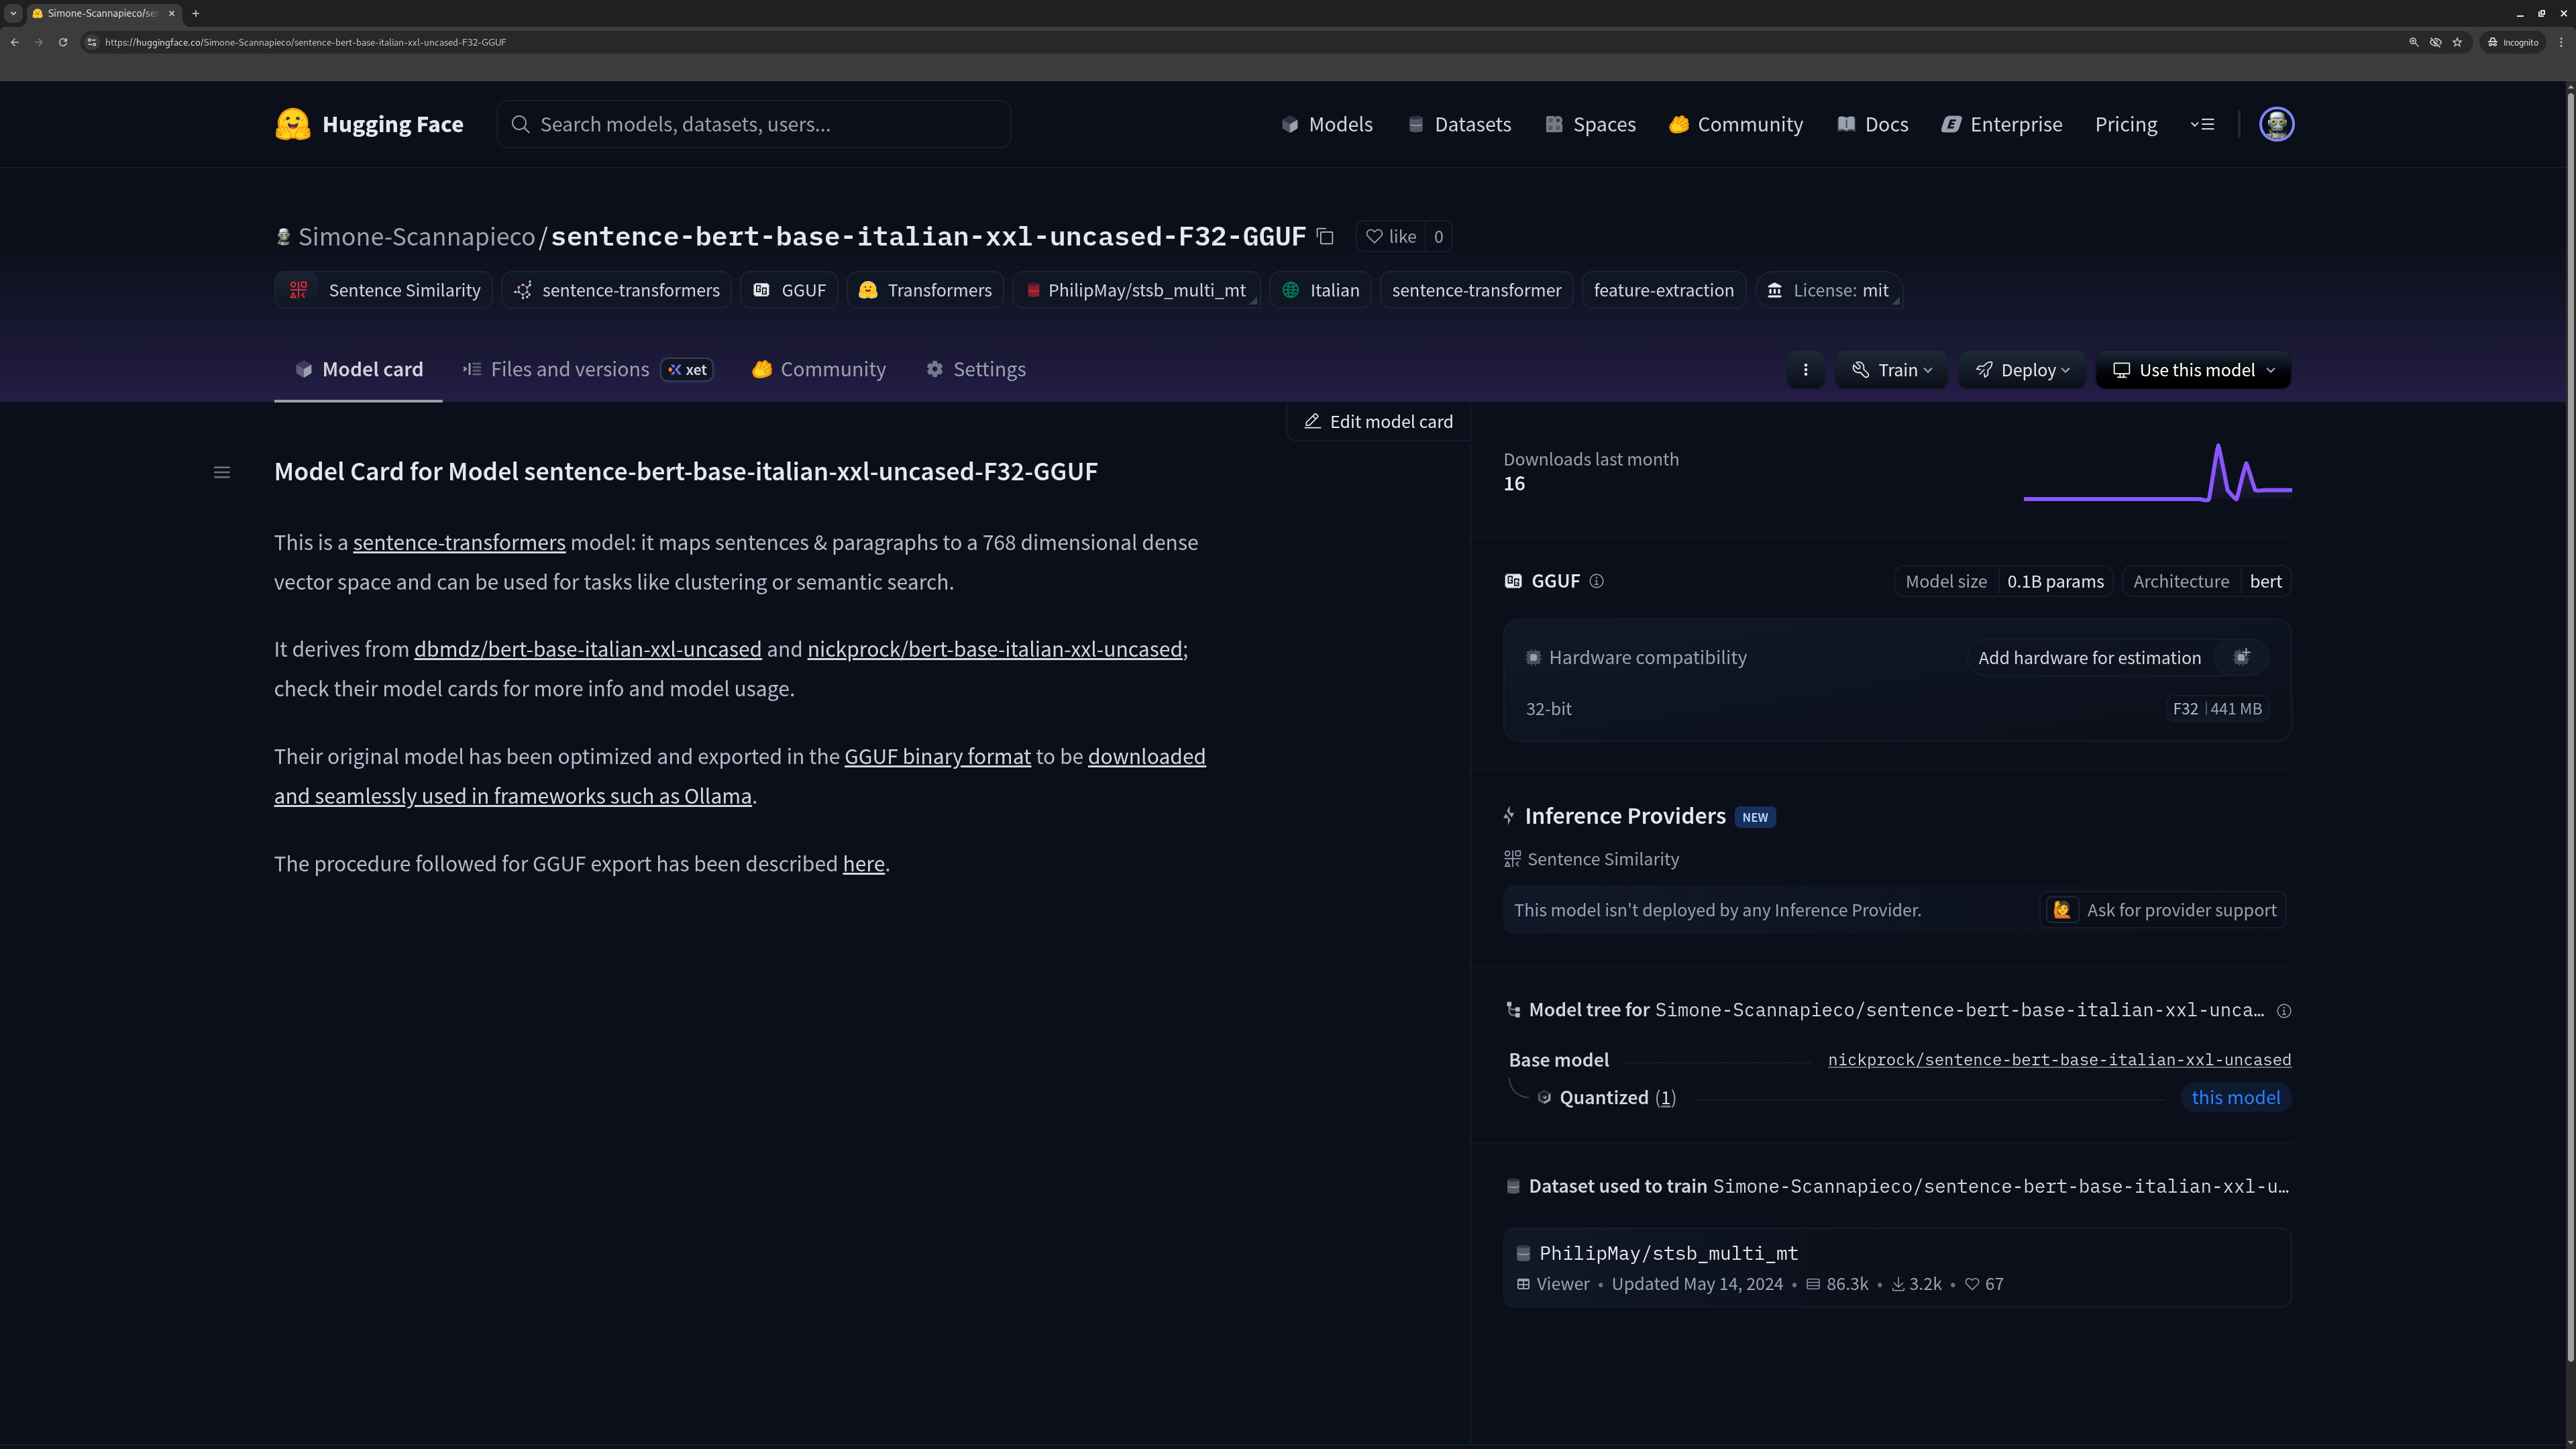
\includegraphics[width=\textwidth, frame]{img/huggingface-model-card.png}
		    \end{figure}
        }
	\end{minipage}
\end{frame}
%
\begin{frame}[t,fragile] \frametitle{Progetto Spring AI}
    \framesubtitle{Variabili di ambiente - Applicativo Spring}
        \begin{block}{\textit{File} \texttt{launch.json}}
			{\tiny\inputminted{json}{code/launch.json}}
    	\end{block}
\end{frame}
%
\begin{frame}[t,fragile] \frametitle{Progetto Spring AI}
    \framesubtitle{Variabili di ambiente - JUnit test}
        \begin{block}{\textit{File} \texttt{settings.json}}
			{\tiny\inputminted{json}{code/settings.json}}
    	\end{block}
\end{frame}
%
\begin{frame}[t,fragile] \frametitle{Progetto Spring AI}
    \framesubtitle{Servizio Docker Qdrant}
        \begin{block}{\textit{File} \texttt{docker-compose.yml}}
			{\tiny\inputminted{yaml}{code/docker-compose.yml}}
    	\end{block}
\end{frame}
%
\begin{frame}[t,fragile] \frametitle{Progetto Spring AI}
    \framesubtitle{Variabili di ambiente servizio Docker Qdrant}
        \begin{block}{\textit{File} \texttt{spring-ai.env}}
			{\tiny\inputminted{text}{code/spring-ai.env}}
    	\end{block}
\end{frame}
%
\begin{frame}[t,fragile] \frametitle{Progetto Spring AI}
    \framesubtitle{RAG}
        \begin{block}{Dipendenze di sistema aggiuntive}
			{\tiny\inputminted{xml}{code/pom.xml}}
    	\end{block}
\end{frame}
%
\begin{frame}[t,fragile] \frametitle{Progetto Spring AI}
    \framesubtitle{RAG}
        \begin{block}{Configurazione applicativo}
			{\tiny\inputminted{yaml}{code/application.yml}}
    	\end{block}
\end{frame}
%
\begin{frame}[t,fragile] \frametitle{Progetto Spring AI}
    \framesubtitle{Script rimozione volumi Docker}
        \begin{block}{\textit{File} \texttt{erase\_llm\_volumes.sh}}
			{\tiny\inputminted{bash}{code/erase_llm_volumes.sh}}
    	\end{block}
        \begin{block}{\textit{File} \texttt{erase\_vector\_store\_volumes.sh}}
			{\tiny\inputminted{bash}{code/erase_vector_store_volumes.sh}}
    	\end{block}
\end{frame}
%
\begin{frame}[t,fragile] \frametitle{Progetto Spring AI}
    \framesubtitle{Prompt per strategia RAG - Italiano}
        \begin{block}{\textit{File} \texttt{get-rag-data-system-ita-prompt.st}}
			{\scriptsize\inputminted{text}{code/get-rag-data-system-ita-prompt.st}}
    	\end{block}
        \vspace*{.3cm}
        \begin{block}{\textit{File} \texttt{get-rag-data-system-eng-prompt.st}}
			{\scriptsize\inputminted{text}{code/get-rag-data-system-eng-prompt.st}}
    	\end{block}
\end{frame}
%
\begin{frame}[t,fragile] \frametitle{Progetto Spring AI}
    \framesubtitle{Configurazione RAG}
        \vspace*{-.7cm}
        \begin{block}{Configurazione Vector Store - I}
			{\tiny\inputminted{java}{code/RAGConfig.java}}
    	\end{block}
\end{frame}
%
\begin{frame}[t,fragile] \frametitle{Progetto Spring AI}
    \framesubtitle{Configurazione RAG}
        \vspace*{-.7cm}
        \begin{block}{Configurazione Vector Store - II}
			{\tiny\inputminted{java}{code/RAGConfig-2.java}}
    	\end{block}
\end{frame}
%
\begin{frame}[t,fragile] \frametitle{Progetto Spring AI}
    \framesubtitle{RAG}
        \vspace*{-.7cm}
        \begin{block}{Componente popolamento Qdrant - I}
			{\tiny\inputminted{java}{code/TextDataLoader.java}}
    	\end{block}
\end{frame}
%
\begin{frame}[t,fragile] \frametitle{Progetto Spring AI}
    \framesubtitle{RAG}
        \vspace*{-.7cm}
        \begin{block}{Componente popolamento Qdrant - II}
			{\tiny\inputminted{java}{code/TextDataLoader-2.java}}
    	\end{block}
\end{frame}
%
\begin{frame}[t,fragile] \frametitle{Progetto Spring AI}
    \framesubtitle{RAG}
        \begin{block}{Interfaccia servizio}
			{\tiny\inputminted{java}{code/RAGService.java}}
    	\end{block}
\end{frame}
%
\begin{frame}[t,fragile] \frametitle{Progetto Spring AI}
    \framesubtitle{RAG}
        \vspace*{-.7cm}
        \begin{block}{Implementazione servizio - I}
			{\tiny\inputminted{java}{code/RAGServiceImpl.java}}
    	\end{block}
\end{frame}
%
\begin{frame}[t,fragile] \frametitle{Progetto Spring AI}
    \framesubtitle{RAG}
        \vspace*{-.7cm}
        \begin{block}{Implementazione servizio - II}
			{\tiny\inputminted{java}{code/RAGServiceImpl-2.java}}
    	\end{block}
\end{frame}
%
\begin{frame}[t,fragile] \frametitle{Progetto Spring AI}
    \framesubtitle{RAG}
        \vspace*{-.7cm}
        \begin{block}{Implementazione servizio - III}
			{\tiny\inputminted{java}{code/RAGServiceImpl-3.java}}
    	\end{block}
\end{frame}
%
\begin{frame}[t,fragile] \frametitle{Progetto Spring AI}
    \framesubtitle{RAG}
    	\vspace*{-.7cm}
        \begin{block}{Implementazione controllore REST}
			{\tiny\inputminted{java}{code/QuestionController.java}}
    	\end{block}
\end{frame}
%
\begin{frame}[t,fragile] \frametitle{Ambiente di sviluppo}
\framesubtitle{Popolamento Vector Store}
	\vspace*{-.5cm}
    {\footnotesize
    \begin{itemize}
        \only<1|handout:1>{\item[\faExclamationTriangle] Verificare la \textit{dashboard} Qdrant (\texttt{http://172.17.0.1:6333/dashboard})
    \end{itemize}
    }
    \vfill
    \begin{minipage}[b]{\textwidth}
		\centering
        \only<1|handout:1>{
		    \begin{figure}[ht]
			    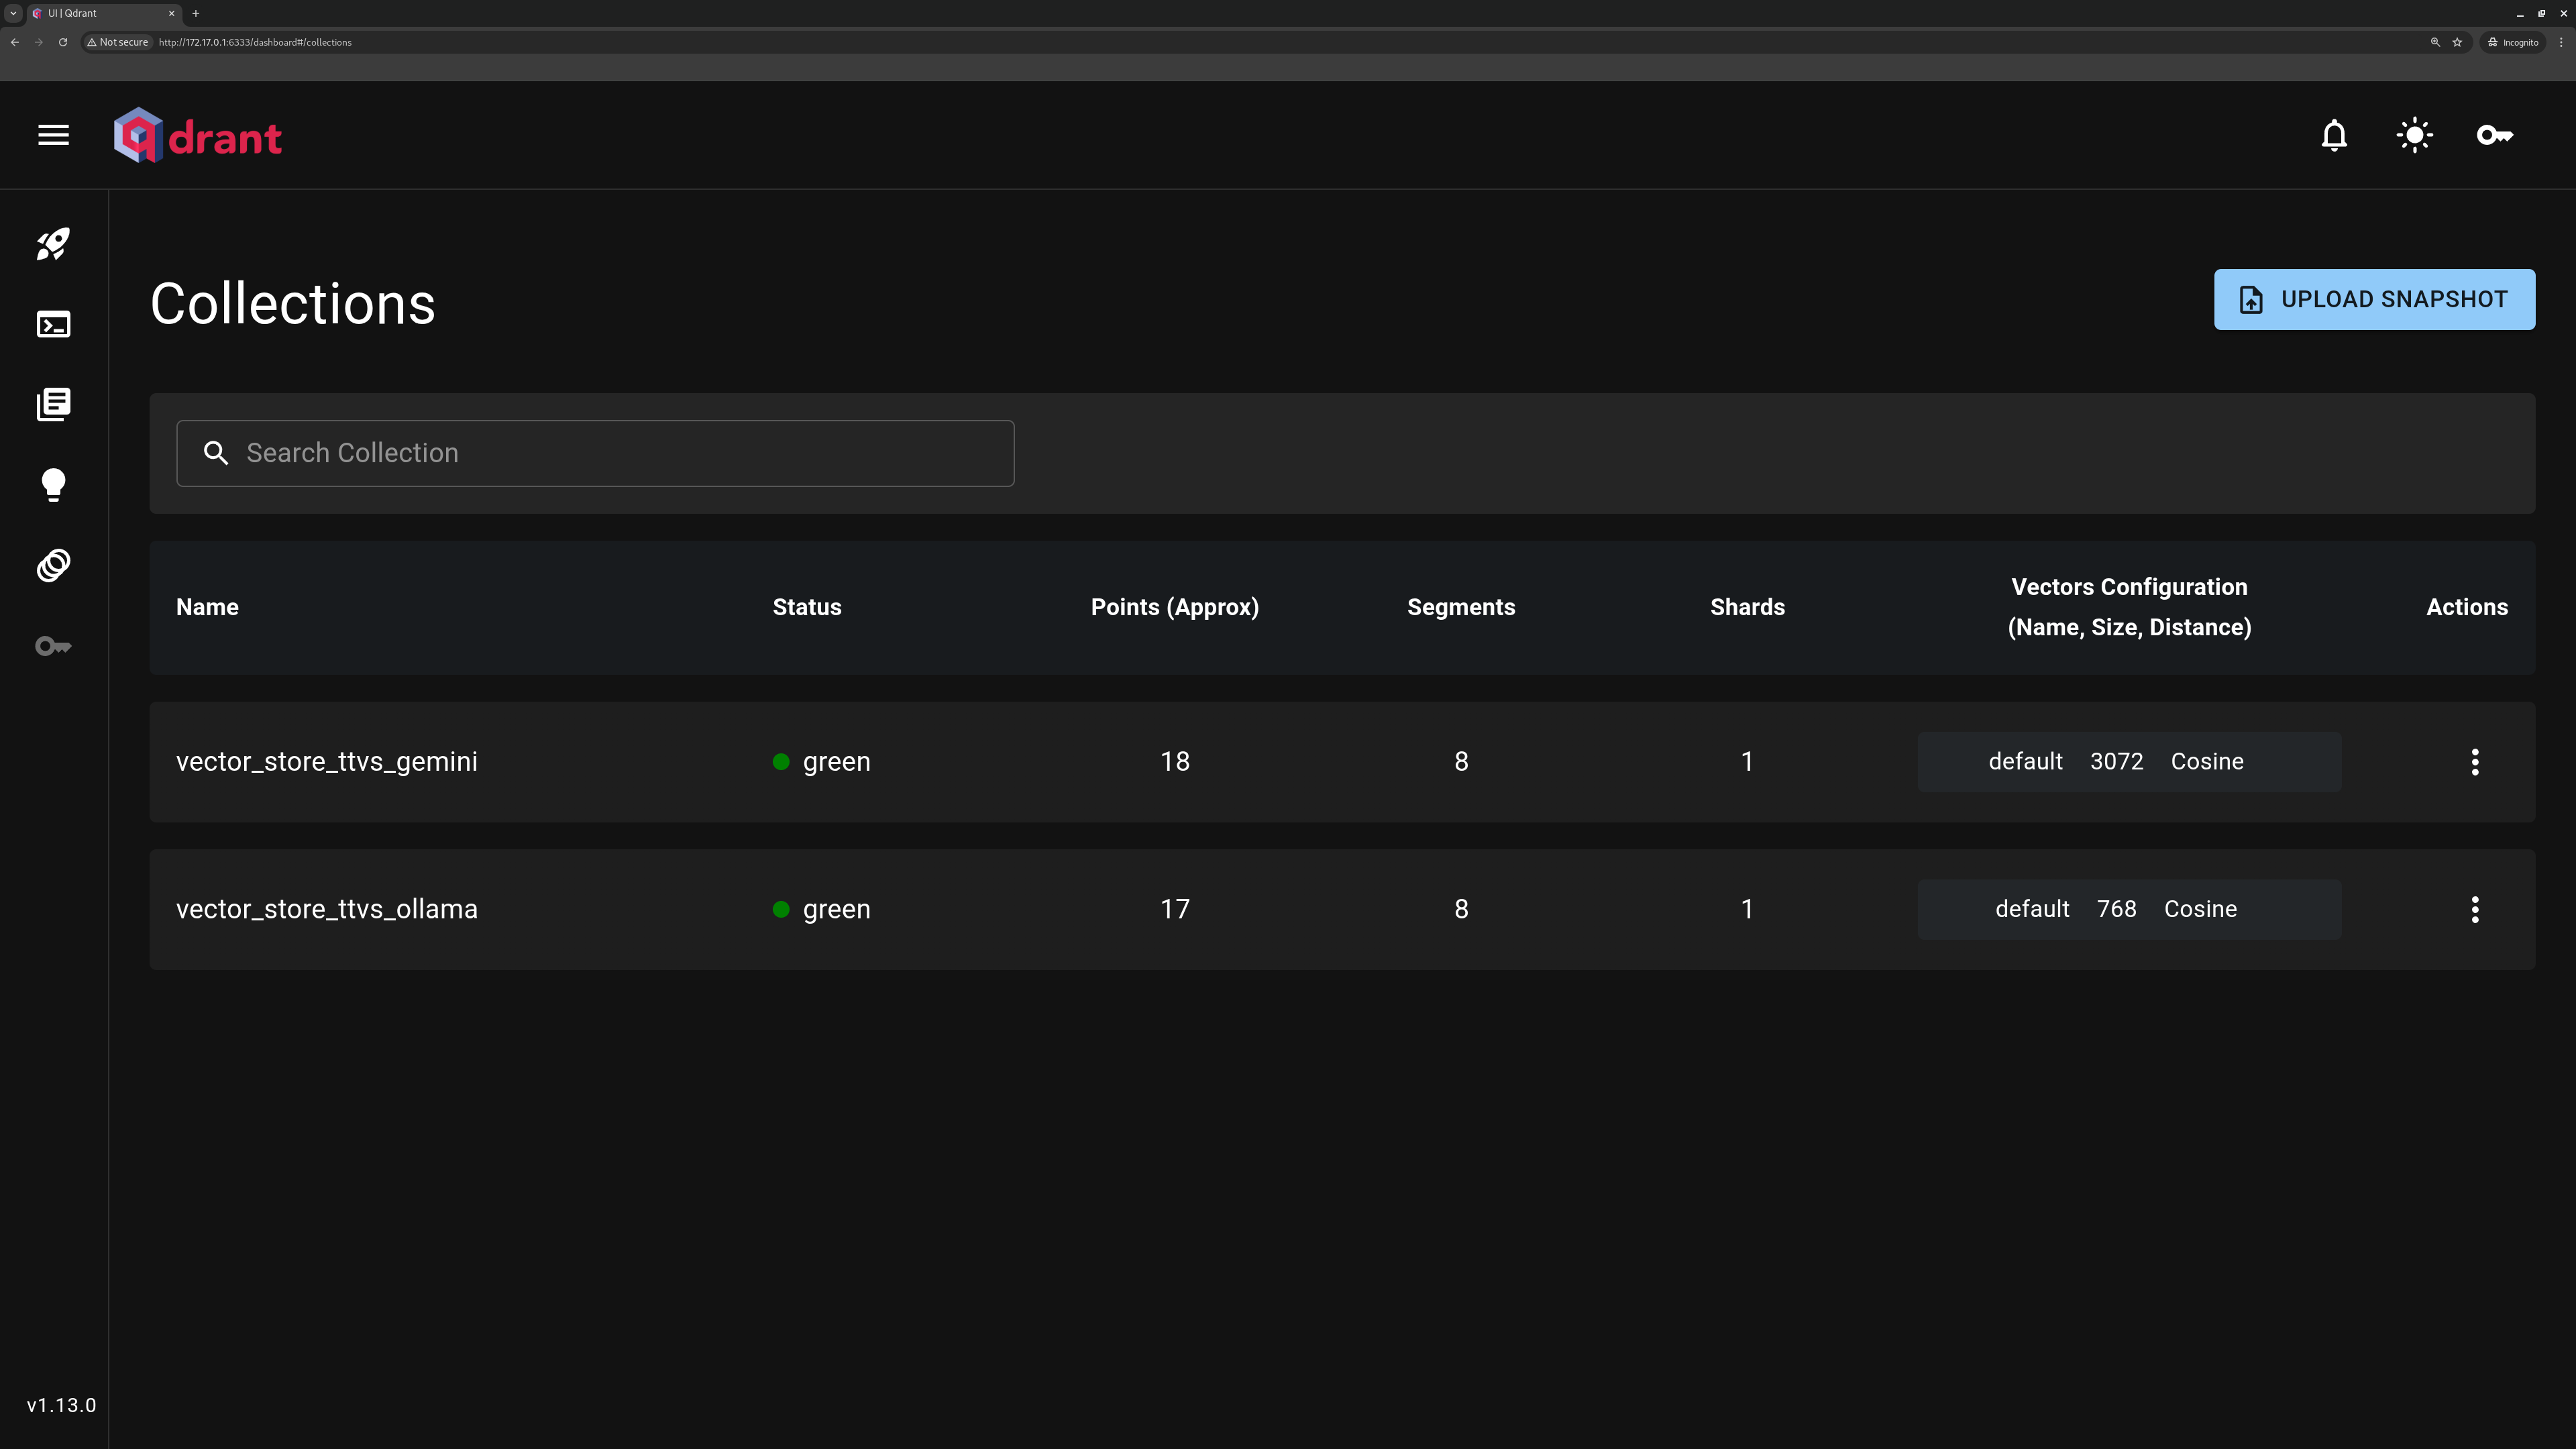
\includegraphics[width=\textwidth, frame]{img/qdrant-dashboard.png}
		    \end{figure}
        }
	\end{minipage}
    }
\end{frame}
%
\begin{frame}[fragile] \frametitle{Codice}
    \framesubtitle{Branch di riferimento}
	\begin{center}
		{\scriptsize \href{https://github.com/simonescannapieco/spring-ai-advanced-dgroove-venis-code.git}{\texttt{https://github.com/simonescannapieco/spring-ai-advanced-dgroove-venis-code.git}}}\\
		\textit{Branch:} \alert{\texttt{7-spring-ai-gemini-ollama-rag-text-to-vector-store}}
	\end{center}
\end{frame}